
\documentclass{beamer}
\setbeamertemplate{navigation symbols}{}

\usepackage{graphicx}
\graphicspath{ {images/} }
\usetheme{Montpellier}
\usepackage{ngerman}
\beamersetuncovermixins{\opaqueness<1>{25}}{\opaqueness<2->{15}}
\begin{document}
\title{Git Introduction mit Windows Github GUI}  
\author{Frederik Wille}

\date{\today} 

\begin{frame}
\titlepage
\end{frame} 

\section{Was ist git?}

\begin{frame}
\frametitle{Was ist git?}
\begin{itemize}
\item Versionskontrolle
\item Contribution Tool
\end{itemize}
\end{frame}

\begin{frame}
\frametitle{Was ist git?}
\begin{itemize}
\item Versionskontrolle
\begin{itemize}
\item Sicherung von fr\"uheren Zust\"anden
\item simultanes Arbeiten an versch. Baustellen
\item Changelogs
\end{itemize}
\item Contribution Tool
\begin{itemize}
\item Parallelisierung
\item Merging
\end{itemize}
\end{itemize}
\end{frame}

%\begin{frame}
%\frametitle {Versions Kontrolle}
%\begin{itemize}
%\item Sicherung von fr\"uheren Zuständen
%\item Arbeiten an versch. Issues
%\item Changelogs
%\end{itemize}
%\end{frame}
%
%\begin{frame}
%\frametitle{Contribution Tool}
%\begin{itemize}
%\item Parallelisierung
%\item Zusammf\"uhrung
%\end{itemize}
%\end{frame}

\begin{frame}
\frametitle{Warum git?}
\begin{itemize}
\item Open Source
\item Performant
\item Dezentralisiert
\item Support am ikum
\end{itemize}
\end{frame}

\section{Vorbereitung}
\subsection{Github}
\begin{frame}
\frametitle{Github}
\begin{minipage}{0.45\textwidth}
\begin{itemize}
\item Github != git
\pause
\item Repos for free
\item sehr gro{\ss}e, aktive Community
\item Studentenpackage
\item Wiki, Issue Tracker, Organisationen und mehr
\end{itemize}
\end{minipage}
\begin{minipage}{0.45\textwidth}
\hfill 
\includegraphics[scale=0.1]{Octocat.png}
\end{minipage}
\end{frame}

\begin{frame}
\frametitle{Github Account}
\begin{itemize}
\item sehr hilfreich
\item kaum Daten n\"otig
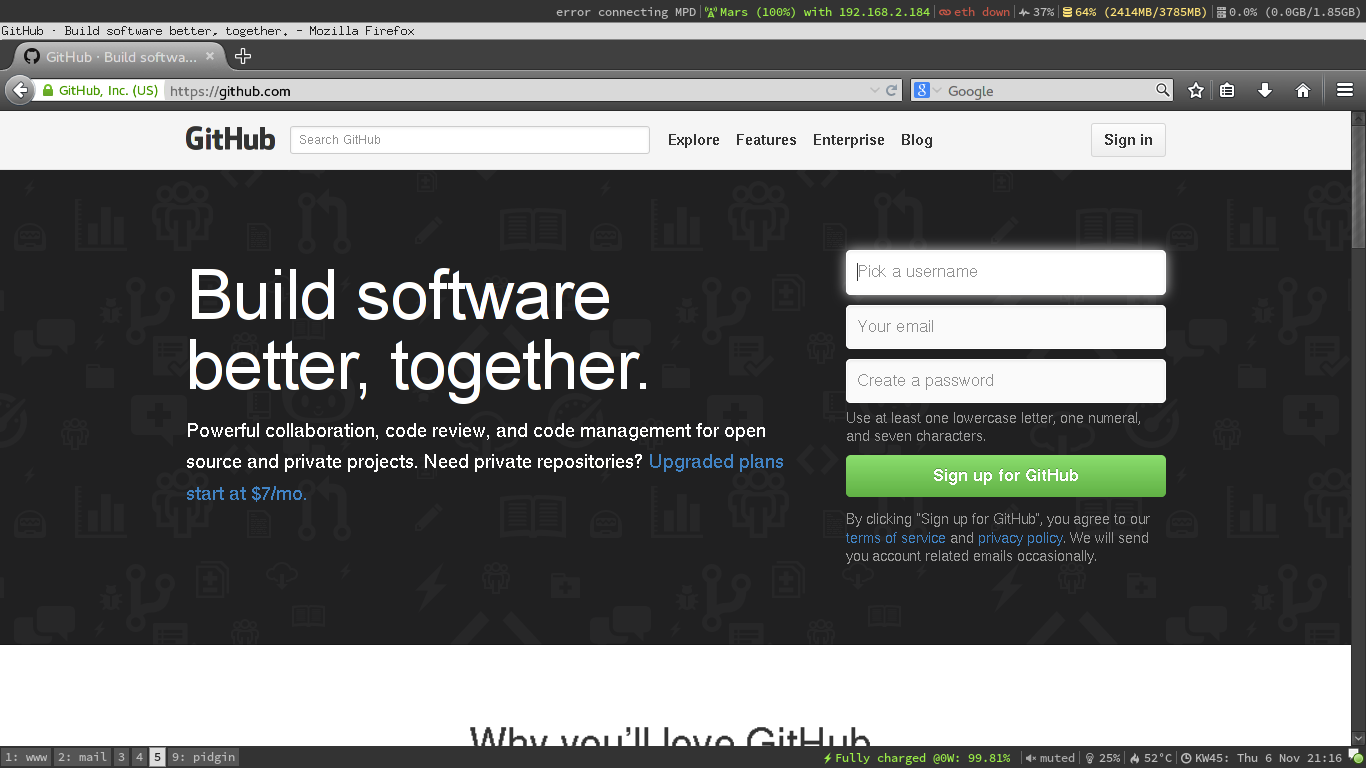
\includegraphics[scale=0.2]{gitreg.png}
\end{itemize}
\end{frame}

\section{Plattformen}
\subsection{So wie man es richtig macht}
\begin{frame}
\frametitle{F\"ur sp\"ater}
\begin{itemize}
\item Linux Shells
\item Git Bash f\"ur Windows\footnote{git-scm.com}
\item SSH Keys erzeugen und nutzen
\end{itemize}
$\Rightarrow$ evtl. KBS, ansonsten fragt Leute oder dieses Internet, von dem alle reden
\end{frame}

\begin{frame}
\frametitle{Windows GUI}
\center
\includegraphics[scale=0.33]{GitWin2.jpg}\\
\small{windows.github.com}
\end{frame}

\section{Anfangen zu arbeiten}
\begin{frame}
\frametitle {Grundlagen}
\begin{itemize}
\item Status der Dateien wird zu jedem Zeitpunkt \"uberwacht
\item bei einem Commit wird der aktuelle Zustand festgehalten
\end{itemize}
\end{frame}

%\begin{frame}
%\frametitle {Dateizust\"ande}
%\center
%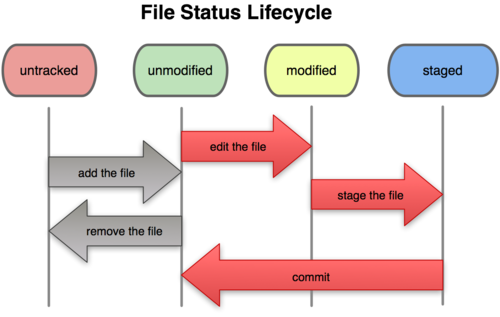
\includegraphics[scale=1]{file_status_lifecycle.png}\\
%\small{https://push.cx/2010/one-fine-git-book-pro-git}
%\end{frame}

%\begin{frame}
%\frametitle{Cheat Sheet}
%\begin{itemize}
%\item git config  --global user.[name,email] 
%\item git clone [url]
%\end{itemize}
%\end{frame}


%\begin{frame}
%\frametitle{Inhaltsverzeichnis}\tableofcontents
%\end{frame} 


%\section{Wo?} 
%\begin{frame}
%\frametitle{Wo?}
%\begin{figure}
%\includegraphics[scale=0.5]{world.png} 
%%\caption{Die Abbildung zeigt ein Beispielbild}
%\end{figure}
%\end{frame}








\end{document}
